\chapter{Brief Overview}\label{Brief Overview}
\section{Background}
To perform task of image captioning we need to first identify objects in an image. That can be done using one of the image labeling model given in next section. These image labeling models generally contains combination of one or more than one types of neural networks which we have discussed in this chapter. Once objects are detected we will generate caption using any of image captioning model.
\section{Different types of neural networks}
Image labeling models are deep learning models that are designed specifically for identifying objects in an image and generate labels based on objects in an image.
\subsection{Recurrent Neural Network (RNN)}

The idea behind RNNs is to make use of sequential information. In normal feedforward networks there is a single input which completely determines the activations of all the neurons through the remaining layers. But if we modify it in such a way that the behaviour of hidden neurons might not just be determined by the activations in previous hidden layers, but also by the activations at earlier times. Indeed, a neuron's activation might be determined in part by its own activation at an earlier time. 

 Here is what a typical RNN looks like:

\begin{figure}[h]
\begin{center}
     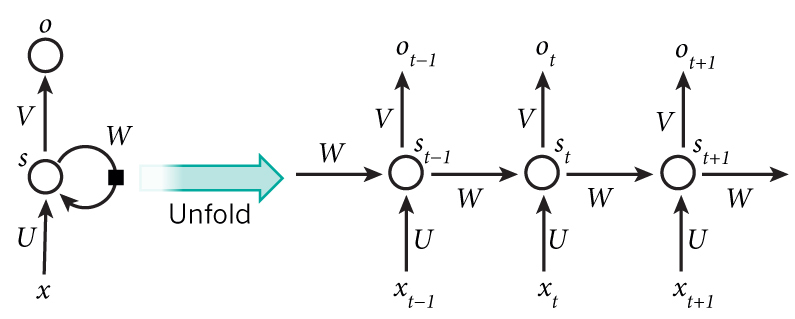
\includegraphics[width=13cm,height=5cm]{img/rnn}
     \caption[Architecture of RNN]{Architecture of RNN \cite{rnnintro}}
     \label{rnn}
\end{center}
\end{figure}
The Figure \ref{rnn} shows a RNN being unrolled (or unfolded) into a full network. By unrolling we simply mean that we write out the network for the complete sequence.

As we can see form Table \ref{imagelabelcompare}, Inception-ResNet provides top-5 error rate of 3.7\% which is even less than average 5\% error rate of human. So we can say that Inception-ResNet provides best accuracy for image labeling task. \\

Similarly for image captioning task previous state of the art model im2text is unable to generate new caption due to its architecture. This problem is solved by Show and Tell(NIC) model. Comparison of both is given in table below.
\begin{table}[H]
\caption{Comparison of different image captioning models}
\label{imagecaptioncompare}
\begin{centering}
\begin{tabular}{|c|c|}
\hline
\textbf{Approch} & \textbf{BLEU Score}\tabularnewline
\hline
\hline
Im2Text \cite{ordonez2011im2text} & 11\tabularnewline
\hline
Show and Tell \cite{7505636} & 28\tabularnewline
\hline
\end{tabular}
\par\end{centering}

\end{table}

In Table \ref{imagecaptioncompare} BLEU score denotes how natural generated sentence is with compared to reference sentence. It is also dependent on sentences used for used for calculating BLEU score so average of multiple BLEU score for same model is used. 